%% LyX 2.1.4 created this file.  For more info, see http://www.lyx.org/.
%% Do not edit unless you really know what you are doing.
\documentclass[english]{article}
\usepackage[T1]{fontenc}
\usepackage[latin9]{inputenc}
\usepackage{babel}
\usepackage{url}
\usepackage{graphicx}
\usepackage[unicode=true,
 bookmarks=false,
 breaklinks=false,pdfborder={0 0 1},backref=section,colorlinks=false]
 {hyperref}
\usepackage{breakurl}

\makeatletter
%%%%%%%%%%%%%%%%%%%%%%%%%%%%%% User specified LaTeX commands.
\date{ }



\usepackage{babel}





\usepackage{babel}


\makeatother

\begin{document}

\title{Proposal for a Project in Data Science}


\author{J�r�my Scheurer, Philipp Miotti, Rob Spaargaren}


\date{\today}

\maketitle

\section*{Project Goal}

The technological progress of our society shapes our daily life in
an unprecedented way and faster than ever before. Internet of Things,
Big Data and Artificial Intelligence have become wide-spread terms.
Agencies for urban planning look for opportunities on how these technologies
can be leveraged for the construction of the cities of tomorrow. They
should support the \textquotedbl{}Smart City vision\textquotedbl{},
which aims at exploiting the most advanced technologies to offer citizens
high quality services. However, the deployment of modern sensors in
many parts of the public space and the modernization of cities to
make them \textquotedbl{}smart\textquotedbl{}, might spur an influx
of wealthy inhabitants, raising the housing prices and hence initiating
the process of gentrification. This leads us to the following important
question, \textquotedbl{}Are Smart Cities gentrified cities?\textquotedbl{}.
The goal of our project is to utilize quantitative measures for both
gentrification and the \textquotedbl{}smartness\textquotedbl{} of
a city, to find out whether Smart cities are more gentrified than
Non-Smart Cities. Or in other words if \textquotedbl{}smartyfing\textquotedbl{}
cities accelerates the process of gentrification with respect to Non-Smart
Cities. This would then provide an answer to the above question: \textquotedbl{}Are
Smart Cities gentrified cities?\textquotedbl{}. We would also like
to provide a tool to predict which cities are expected to be gentrified
in the near future based on its \textquotedbl{}smartness\textquotedbl{}(assuming
that there actually is a positive correlation between the \textquotedbl{}smartness\textquotedbl{}
and the gentrification)\\



\subsection*{Approach}

To achieve this goal, a quantitative measure for gentrification is
needed, which requires knowledge of the nature of the process. The
process involves wealthier residents moving into an area that was
previously dominated by residents of low social classes. The new,
richer residents invest in the neighbourhood to renovate it until
it conforms to the taste of its higher class residents. This way,
living costs rise, so the poorer, lower class residents are forced
to move out until the neighbourhood has turned into a middle- to upper
class area. \\


Thus, gentrification causes changes in both the nature of residents
of an area, where poor, low-class residents are replaced by wealthier,
middle- to upper- class residents, and the nature of the neighbourhood
itself, where housing prices and living costs rise and the area will
become safer with more public green, parks and more schools. The latter
part is not always indicative of gentrification, however, but could
be due to a number of other factors like a change of policy by the
city government, and can be subjective of nature. Also, of all the
changes in characteristics of the residents (smaller families, higher
education, higher percentage of foreigners), an increase of income
is the most indicative and least subjective sign of the transition
to a higher social class. Therefore, to measure gentrification in
a quantitative manner, it makes the most sense to construct a measure
based on general income. This is in line with research on gentrification
({[}1{]}). Thus, our approach to the project is as follows: 
\begin{enumerate}
\item Retrieve data on the average income of inhabitants of a certain city
part. We do this process for a to be determined selection of both
\textquotedbl{}Smart Cities\textquotedbl{} and \textquotedbl{}Non-Smart
Cities\textquotedbl{}. 
\item Find or construct a measure which allows us to summarize the gentrification
of a city with an index. To find such a measure, we have to analyse
the average income of different neighbourhoods of a city and investigate
the relation between those neighbourhoods to find an \textquotedbl{}index
of gentrification\textquotedbl{}. 
\item Relate the \textquotedbl{}index of gentrification\textquotedbl{} to
how \textquotedbl{}smart\textquotedbl{} a city is. This will allow
us to answer the projects question \textquotedbl{}Are smart cities
gentrified cities?\textquotedbl{}. 
\end{enumerate}

\subsection*{Challenges}

The challenges of this Project will be the following: 
\begin{enumerate}
\item Finding cities where sufficient data is available on income of their
different neighbourhoods. 
\item Collecting this data into one, clean database. 
\item The most challenging part of the project will be to construct a model
which takes the average income of neighbourhoods and yields a \textquotedbl{}gentrification
index\textquotedbl{}. 
\end{enumerate}

\section*{Data collection}

For this project, we have chosen to utilize publicly available data
sources for the data collection of this project. First of all, we
will try to find out what defines Smart Cities and which cities today
are already considered to be smart. To give an indication of the smartness
of a city, we will use two publicly available rankings of cities across
the globe. The higher a city is on both lists, the smarter it is.
One list, published by the IESE Business School of the Universtiy
of Navarra {[}2{]}, is based on 66 different indicators, subdivided
in 10 dimensions: Human capital, social cohesion, economy, public
management, governance, mobility and transportation, environment,
urban planning, international outreach and techonology. Our other
source is the Easypark group {[}3{]}, an international group specialising
in implementation of smart parking in cities, who have created a ranking
based on transport and mobility, sustainability, governance, innovation
economy, digitalisation, living standards and expert perception. From
these rankings, we will choose cities that are classified as smart,
and use their ranking on both lists as a measure of their smartness.
Subsequently, we need to choose non-smart cities to compare these
cities to. \\


These non-smart cities must be chosen to provide optimal conditions
to compare gentrification between those cities and the smart cities.
We are only interested in the effect of the smartness of a city on
gentrification. Therefore, the selection of non-smart cities should
eliminate as many factors as possible which could affect the rate
of gentrification as well, such as size of the city and city-wide
average income. This provides us with the best possible opportunity
to compare the gentrification between these cities and the smart cities.
\\


After selection of cities to be used in this project is complete,
we will proceed by collecting data on the average income of all neighbourhoods
of these cities. We are confident that, especially in the USA, we
will be able to retrieve such data from online, publicly available
sources. There has been a considerable amount of research on gentrification
in US cities (e.g.\ {[}1{]},{[}4{]}) which used publicly available
census data. We will retrieve this data and collect it into one common
database, where we can analyse it. \\



\section*{Data Science approach}

We have chosen to use a data science approach to answer the main question
of this project for several reasons. One reason is, that there is
a lot of publicly available data which we can leverage. As this project
wants to investigate global trends in different cities of the world,
approaches of interviewing, observing or experimenting would be impossible
to conduct. We are also confident, that a large amount of specific
data will make us able to see some general trends. Naturally more
data is not always better, but if we find the right kind of data (as
described in the section \textquotedbl{}Data collection\textquotedbl{})
we will be able to see if there are actual correlations between gentrification
and the smartness of a city. Factors that only play a role for specific
cities (in other words \textquotedbl{}noise\textquotedbl{}) will vanish
the more data we have. Additionally, if we perceive the problem from
a statistical perspective, we are trying to find out correlations
between gentrification and the process of becoming a Smart City. This
can, from a statistical perspective, only be answered with analysis
of data. \\


We will specifically apply a form of Machine Learning to determine
the \textquotedbl{}gentrification index\textquotedbl{} from the average
income of the inhabitants of certain city parts. Although we only
have the average income of city neighbourhoods available as data,
there is a large amount of subtle information hidden in this data,
which we can use. These are things such as the link between geographic
location and average income, the change in the average income over
time, the closeness of different city parts like the city centre,
etc. Retrieving this information from the available data is not a
trivial task and we think that a Machine Learning approach is the
most efficient way of utilizing the available data. \\



\section*{Outcome of our project}

We expect that our project will result in a greater understanding
of what influence the transition from an ordinary city to a smart
city has on the demographic development of a city. Our results will
most likely either look like the graphs drawn in Figure 1, or the
results will look more randomized if no correlation between gentrification
and the development from an ordinary to a smart city can be found.
Understanding the influence of developing towards a smart city can
help policy makers and urban city planners to incorporate precautionary
measures into Smart City projects, to prevent gentrification.

\begin{figure}[h]
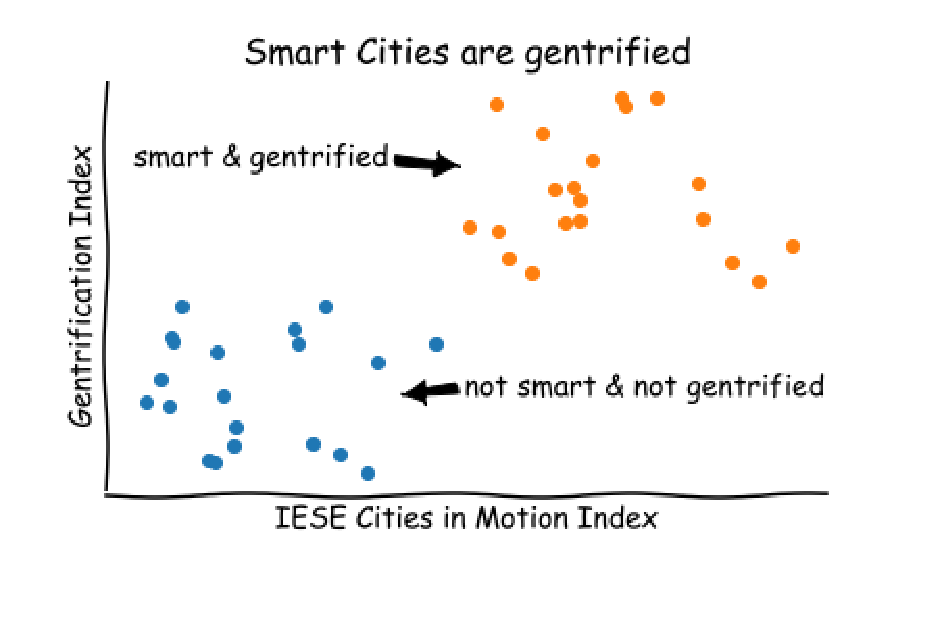
\includegraphics[scale=0.41]{postive_corr}\hfill{}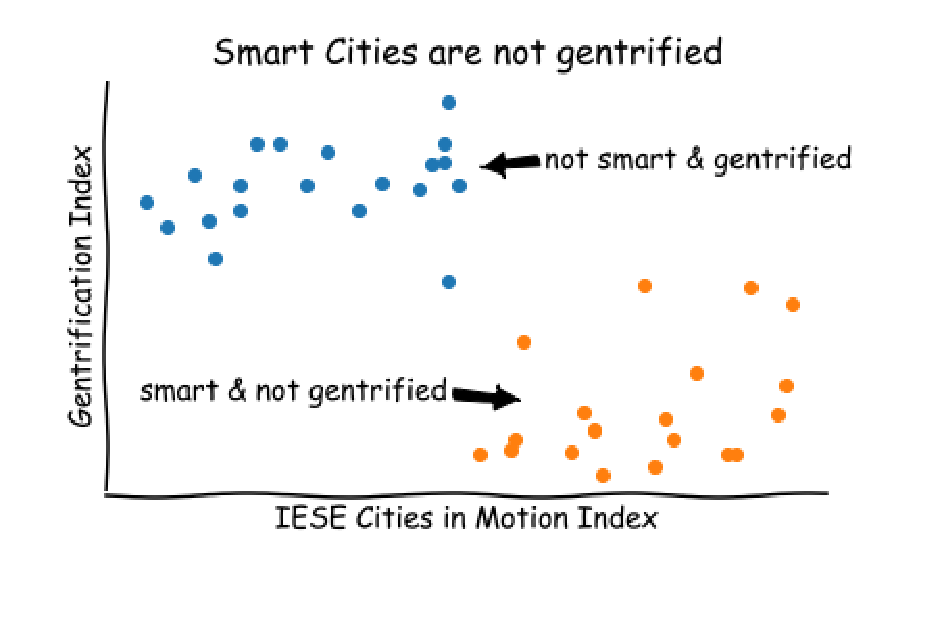
\includegraphics[scale=0.41]{negative_corr}

\centering{}\caption{Possible correlations between gentrification and smartness of a city.}
\end{figure}



\section*{Bibliography}
\begin{enumerate}
\item Ding, L., Hwang, J., Divringi, E.\ (2016). \emph{Gentrification and
residential mobility in Philadelphia}. Regional Science and Urban
Economics, 61, \emph{38-51}. 
\item Berrone, P., Ricart., J.E.\ (2017). \emph{IESE Cities in Motion Index}.
Retrieved from IESE website: \url{http://www.iese.edu/research/pdfs/ST-0396-E.pdf} 
\item Easypark group 2017 Smart Cities Index (n.d.). Retrieved from \url{https://easyparkgroup.com/smart-cities-index/} 
\item Maciag, M.\ (2015, February). \emph{Gentrification in America Report}.
Retrieved from \begin{sloppypar}\url{http://www.governing.com/gov-data/gentrification-in-cities-governing-report.html}
\end{sloppypar} \end{enumerate}

\end{document}
